\documentclass[12pt]{article}
\usepackage{import}
\usepackage{preamble}
%\usepackage{fourier}

%hspace before small will move the keywords around
\providecommand{\keywords}[1]
{
    \hspace*{0pt}\small	
  \textbf{\textit{Keywords--}} #1
}

\title{Information and Entropy}
\renewcommand{\maketitlehookb}{\centering Mathematical Physics Lab\\
Colorado State University}
\author{Colin Roberts}
\date{September 2019}


\begin{document}

% Title Page
\begin{titlingpage}
    \maketitle
    \vfill
    \begin{abstract}
        What does one mean when using the word information? Given some type of system, how much information does it contain? How about entropy? Does this physical quantity relate to a mathematical quantity of information? In this talk, we seek to answer the above questions in a (hopefully) intuitive manner. The measure of information in a system can be properly represented by a family of logarithmic functions which we arrive at using heuristic and logical arguments. Following, we explore the role of information in thermodynamical systems and its direct relationship to entropy.
        
        I will base much of the mathematics off of Claude Elwood Shannon's wonderful paper titled "A Mathematical Theory of Communication." If the topic at hand interests you, please consider exploring this piece. The physics covered can be found in many different thermodynamics or statistical mechanics textbooks.
        
        
    \end{abstract}
    %\vspace*{10pt}
    \keywords{measurable, idk, entropy probably}
\end{titlingpage}

% \section*{Outline}
% \begin{enumerate}[1.]
%     \item Introduce smooth manifolds by building up from topological spaces.
%     \item Define bundles generally and then introduce the canonical bundles $TM$ and $T^*M$.
%     \item Realize the space of sections of $TM$ and $T*M$ form a $C^\infty(M)$-module.
%     \item Build the tensor product of bundles and tensor product of the spaces of sections.
%     \item Show the examples of the (0,2)-tensor bundle and the $k$-exterior power bundle and their sections.
%     \item Mention the tensor algebra and quotients and consider the construction on $M$.
% \end{enumerate}

\section{Introduction}

\subsection{Motivation}
Manifolds are spaces that locally behave like $\R^m$.  In essence, they seek to generalize some of the properties of $\R^m$ but with nontrivial topology.  This nontrivial topology is important in many applications.  For example, consider the convective flow in the Earth's atmosphere or even a bead sliding on a circular loop. Both are examples of dynamical problems on manifolds.

The goal of differential geometry is to understand the local geometrical features of manifolds via calculus. One idea is to study real valued functions on manifolds in hopes of noticing differences in the geometric structure.  An example of this would be a Morse function which can detect topological features.  To investigate local geometry, we work with more general functions called tensors. Smooth manifolds admit some natural tensors which can give the manifold shape. For example, attaching a metric tensor allows one to distinguish the unit 2-sphere from the surface of a bumpy potato.

The metric tensor is a specific type of tensor field attached to a Riemannian manifold.  Tensor fields are smoothly varying tensors defined on vector spaces attached at each point on a manifold.  These vector spaces can be glued together in a structure called a vector bundle using the smooth structure on the underlying manifold. With the notion of a smooth map between manifolds, one can then define tensor fields as smooth sections of an appropriate tensor product of vector bundles.  

\subsection{Preliminaries}
% Throughout, I will use the following notation and conventions:
% \begin{itemize}
%     \item $V$ represents a finite dimensional vector space of dimension $n$.  $V^*$ represents its dual.
%     \item $\{e_1,\dots,e_n\}$ will be a basis for $V$ and it will likely satisfy nice properties when needed (i.e., it is orthonormal).  I will use superscripts to denote dual elements, and it follows that $\{e^1,\dots,e^n\}$ is the canonical dual basis, that is, the basis satisfying
%     \[
%     e^i (e_j) = \delta^i_j = \begin{cases}
%     1 & i=j\\
%     0 & \textrm{otherwise}
%     \end{cases}.
%     \]
%     \item $M$ will represent an $m$ dimensional (smooth, Riemannian, etc.) manifold with $T_pM$ as the tangent space at the point $p$ and $TM$ the tangent bundle.  Similarly, $T^*_pM$ will be the cotangent space at the point $p$ and $T^*M$ the cotangent bundle.
%     \item Working in local coordinates $(U,\phi)$ may happen, and in this case we take a basis of $T_U M$ to be $\left\{\frac{\partial}{\partial x^1}, \dots,\frac{\partial}{\partial x^m}\right\}$.  Or more succinctly, one may write $\{\partial_1,\dots \partial_m\}$ which proves to be nice when we are ignoring the fact that tangent vectors are differential operators.
    
%     Similarly, we let $T^*_UM$ have the canonical dual basis $\{dx^1,\dots,dx^m\}$ which satisfies
%     \[
%     dx^i (\partial_j)\coloneqq \frac{\partial x^i}{\partial x^j} = \delta^i_j.
%     \]
%     \item It's nice to reference the space $\R^{r,l,t}$ as the vector space $\R^{r+l+t}$ with basis $\{e_1,\dots,e_r,e_{r+1},$ $\dots,e_{r+l},e_{r+l+1}\dots,e_{r+l+t}\}$ and quadratic form $Q$ satisfying
%     \[
%     Q(e_i) = \begin{cases}
%     -1 & i = 1,\dots, r\\
%     0 & i = r+1,\dots, r+l\\
%     1 & i = r+l+1,\dots,r+l+t
%     \end{cases}.
%     \]
%     \item Since $V$ will be finite dimensional, we also have that $V^{**}\cong V$.  This will be used without constantly mentioning this fact.  Of course, we realize this isomorphism by allowing
%     \[
%     e_i(e^j)=e^j(e_i) = \delta^j_i.
%     \]
% \end{itemize}

% One should be aware that many of the definitions I choose here can be generalized.  For example, fiber bundles generalize vector bundles and the base space need not be a manifold.  It follows that sections can be generalized a bit as well. 

To create smooth tensor fields we must first build the notion of a smooth manifold. The first step is to define a \emph{topological manifold}.  These are topological spaces which are locally equivalent (\emph{homeomorphic}) to $\R^m$.  
\begin{df}{Homeomorphism}{homeo}
Let $M\equiv(M,\opens_M)$ and $N\equiv(N,\opens_N)$ be two topological spaces.  We say that $M$ is \textbf{homeomorphic} to $N$ if there exists a continuous bijection $f\colon M \to N$ with continuous inverse.
\end{df}

With this notion, we can define topological manifolds.  The addition of smooth structure will follow.

\begin{df}{Topological Manifolds}{top_mfd}
Let $M\equiv(M,\opens)$ be a (second countable) Hausdorff topological space.  We say that $M$ is an \textbf{$m$-dimensional topological manifold} if $M$ is locally homeomorphic to $\R^m$. That is, each $U\in \opens$ is homeomorphic to some open set $X\subset \R^m$ with the metric topology.
\end{df}

\begin{rmk}{Other Notions of Manifolds}{other_notions}
Often, manifolds come with other properties.  However, we really don't need any others.  The Hausdorff property isn't asking much and prevents some pathological spaces such as the line with two origins. The second countable property allows for integration.
\end{rmk}

This definition gives us the notion of a manifold that is familiar.  However, we wish to add a \emph{smooth structure} to the space so that we can develop a richer geometry. Roughly speaking, we must upgrade the notion of a homeomorphism to that of a \emph{diffeomorphism}. This allows us to use the smoothness of $\R^m$ to do calculus on a manifold.

\begin{df}{Smooth Structure}{smooth_struc}
Let $M$ be a an $m$-dimensional topological manifold.  We call $M\equiv(M,\opens,\atlas)$ a \textbf{smooth manifold} if we can place a smooth structure on $M$ (the addition of $\atlas$). The smooth structure is given by the following.
\begin{itemize}
    \item \textbf{Coordinate charts}. Given $U_\alpha\in \opens$ we have a $(U_\alpha,\varphi_\alpha)$ with $\varphi \colon U\subset M \to X \subset \R^m$.
    \item Smooth transitions. That is, given overlapping charts $(U_\alpha,\varphi_\alpha)$ and $(U_\beta,\varphi_\beta)$ with $U_\alpha \cap U_\beta = U_{\alpha \beta} \neq \emptyset$ we have that the map
    \[
    \varphi_{\alpha \beta} = \varphi_\beta \circ \varphi_\alpha^{-1} \colon \varphi(U_{\alpha \beta}) \subset \R^m \to \R^m
    \]
    is smooth as a map from $\R^m$ to $\R^m$.  
    \item We collect all possible compatible charts into a collection called an \textbf{atlas} $\atlas$ which gives us the smooth structure.
\end{itemize}
The degree of smoothness depends on the differentiability class of the transitions.  That is, they could be $C^k$ for $k=0,\dots,\infty$, or analytic. Here we choose $C^\infty$ and by manifold refer to $C^\infty$-smooth manifolds for the remainder of this talk.
\end{df}

The provided definition of a smooth manifold may not seem intuitive at first glance.  However, the naming scheme used is rather helpful as we can picture charts as pages of an atlas of Earth. The interpretation of the charts can be seen pictorially.

\begin{fig}{Coordinate Charts}{coord_charts}
\begin{figure}[H]
    \centering
    \begin{overpic}[width=0.8\textwidth]{TACA_2019/coordinate_charts_manifold.png}
    \put (39,61) {\Large$U_\alpha$}
    \put (70,57) {\Large$U_\beta$}
    \put (12,65) {\LARGE$M$}
    \put (20,35) {\Large$\varphi_\alpha$}
    \put (73,30) {\Large$\varphi_\beta$}
    \put (22,3) {\Large$\R^m$}
    \put (60,3) {\Large$\R^m$}
    \put (38,32) {\Large$\varphi_{\alpha \beta}$}
    \put (38,18) {\Large$\varphi_{\beta \alpha}$}
    \end{overpic}
    \caption{A manifold $M$ with overlapping charts $(U_\alpha,\varphi_\alpha)$ and $(U_\beta,\varphi_\beta)$ and transition functions $\varphi_{\alpha \beta}$ and $\varphi_{\beta \alpha}$.}
    \label{fig:my_label}
\end{figure}
\end{fig}

Finally, we need to define a more general notion of smoothness if we wish to do calculus on manifolds.  Since we understand calculus with functions from $\R^m$ to $\R^n$, we build from there.  

\begin{df}{Smooth Map}{smooth_map}
Let $f\colon M \to N$ be a map from an $m$-dimensional manifold $M$ to an $n$-dimensional manifold $N$.  Let $(\varphi, U)$ and $(\psi, V)$ be charts on $M$ and $N$ respectively with $f\colon U \to V$.  We say that $f$ is a \textbf{smooth map} if
\[
\psi \circ f \circ \varphi^{-1} \colon \varphi(U)\subset \R^m \to \psi(V)\subset \R^n
\]
is smooth.
\end{df}

\section{Gluing Together Tensors}

\subsection{Vector Bundles}
One way to add more structure to a manifold is to consider \emph{bundles}  and their respective \emph{sections}. Vector bundles seek to glue together vector spaces over a manifold and sections of bundles play the role of what are referred to as fields or global functions.  For example, one may wish to attach a vector field on a manifold to define a dynamical system. In this language, a vector field is a sections of the tangent bundle. \emph{My apologies to those offended by the name ``field" being used here!}

\begin{df}{Vector Bundles}{vec_bundle}
A (finite dimensional) \textbf{vector bundle on $M$} is a triple $E\equiv (E,M,\pi)$.
\begin{itemize}
    \item $E$ is the \textbf{total space}.
    \item $M$ is a smooth manifold called the \textbf{base space}.
    \item $\pi$ is the \textbf{projection map} $\pi \colon E \to M$. 
\end{itemize}
The relevant vector space is fibered over $E$ as $V=\pi^{-1}(x)$ for $x\in M$. Locally, we have that $E$ looks like a product $U\times V$ with $U\in \opens$. \\

\emph{Warning:} this does not mean every vector bundle is a product $M\times V$.  If it is, we call the bundle \textbf{trivial}.  \\

\emph{Note:} When referring to vector bundles, I will restrict to the case where the fibers, $V$, are finite dimensional.
\end{df}

\begin{rmk}{Bundles are Manifolds}{bundles_manifolds}
Any vector bundle $E$ is itself a smooth manifold.  This fact allows us to define \emph{smooth sections} by using the definition of a smooth map.
\end{rmk}

Every smooth manifold comes equipped with a natural bundle.  This bundle is the \emph{tangent bundle}. It is a collection of the \emph{tangent spaces} that are attached at each point of a manifold.

\begin{df}{Tangent Space}{tangent_space}
Consider a curve $\position \colon (-\epsilon,\epsilon)\to M$ with $\position(0)=x$.  Then we define the \textbf{tangent space at $x$}, $T_xM$, to be the set of equivalence classes of tangent vectors $\velocity(0)$ to curves $\position$. 
\end{df}
The tangent space is made up of differential operators.  The dimension of the tangent space describes the different directions one can differentiate in.  If $M$ is an $m$-dimensional manifold, then $T_xM$ is an $m$-dimensional vector space for each $x\in M$.

It's worth seeing what this looks like pictorially.  One can imagine a curve $\position$ that passes through the point $x$ which has a tangent vector $\velocity(0)=\mathbf{v}$.  If we were to take every possible curve through $x$, then the set of velocity vectors at $x$ defines the tangent space $T_xM$.

% Tangent Space Pictures

\begin{fig}{Tangent Space $T_xM$}{tangent_space_txm}
\begin{figure}[H]
    \centering
    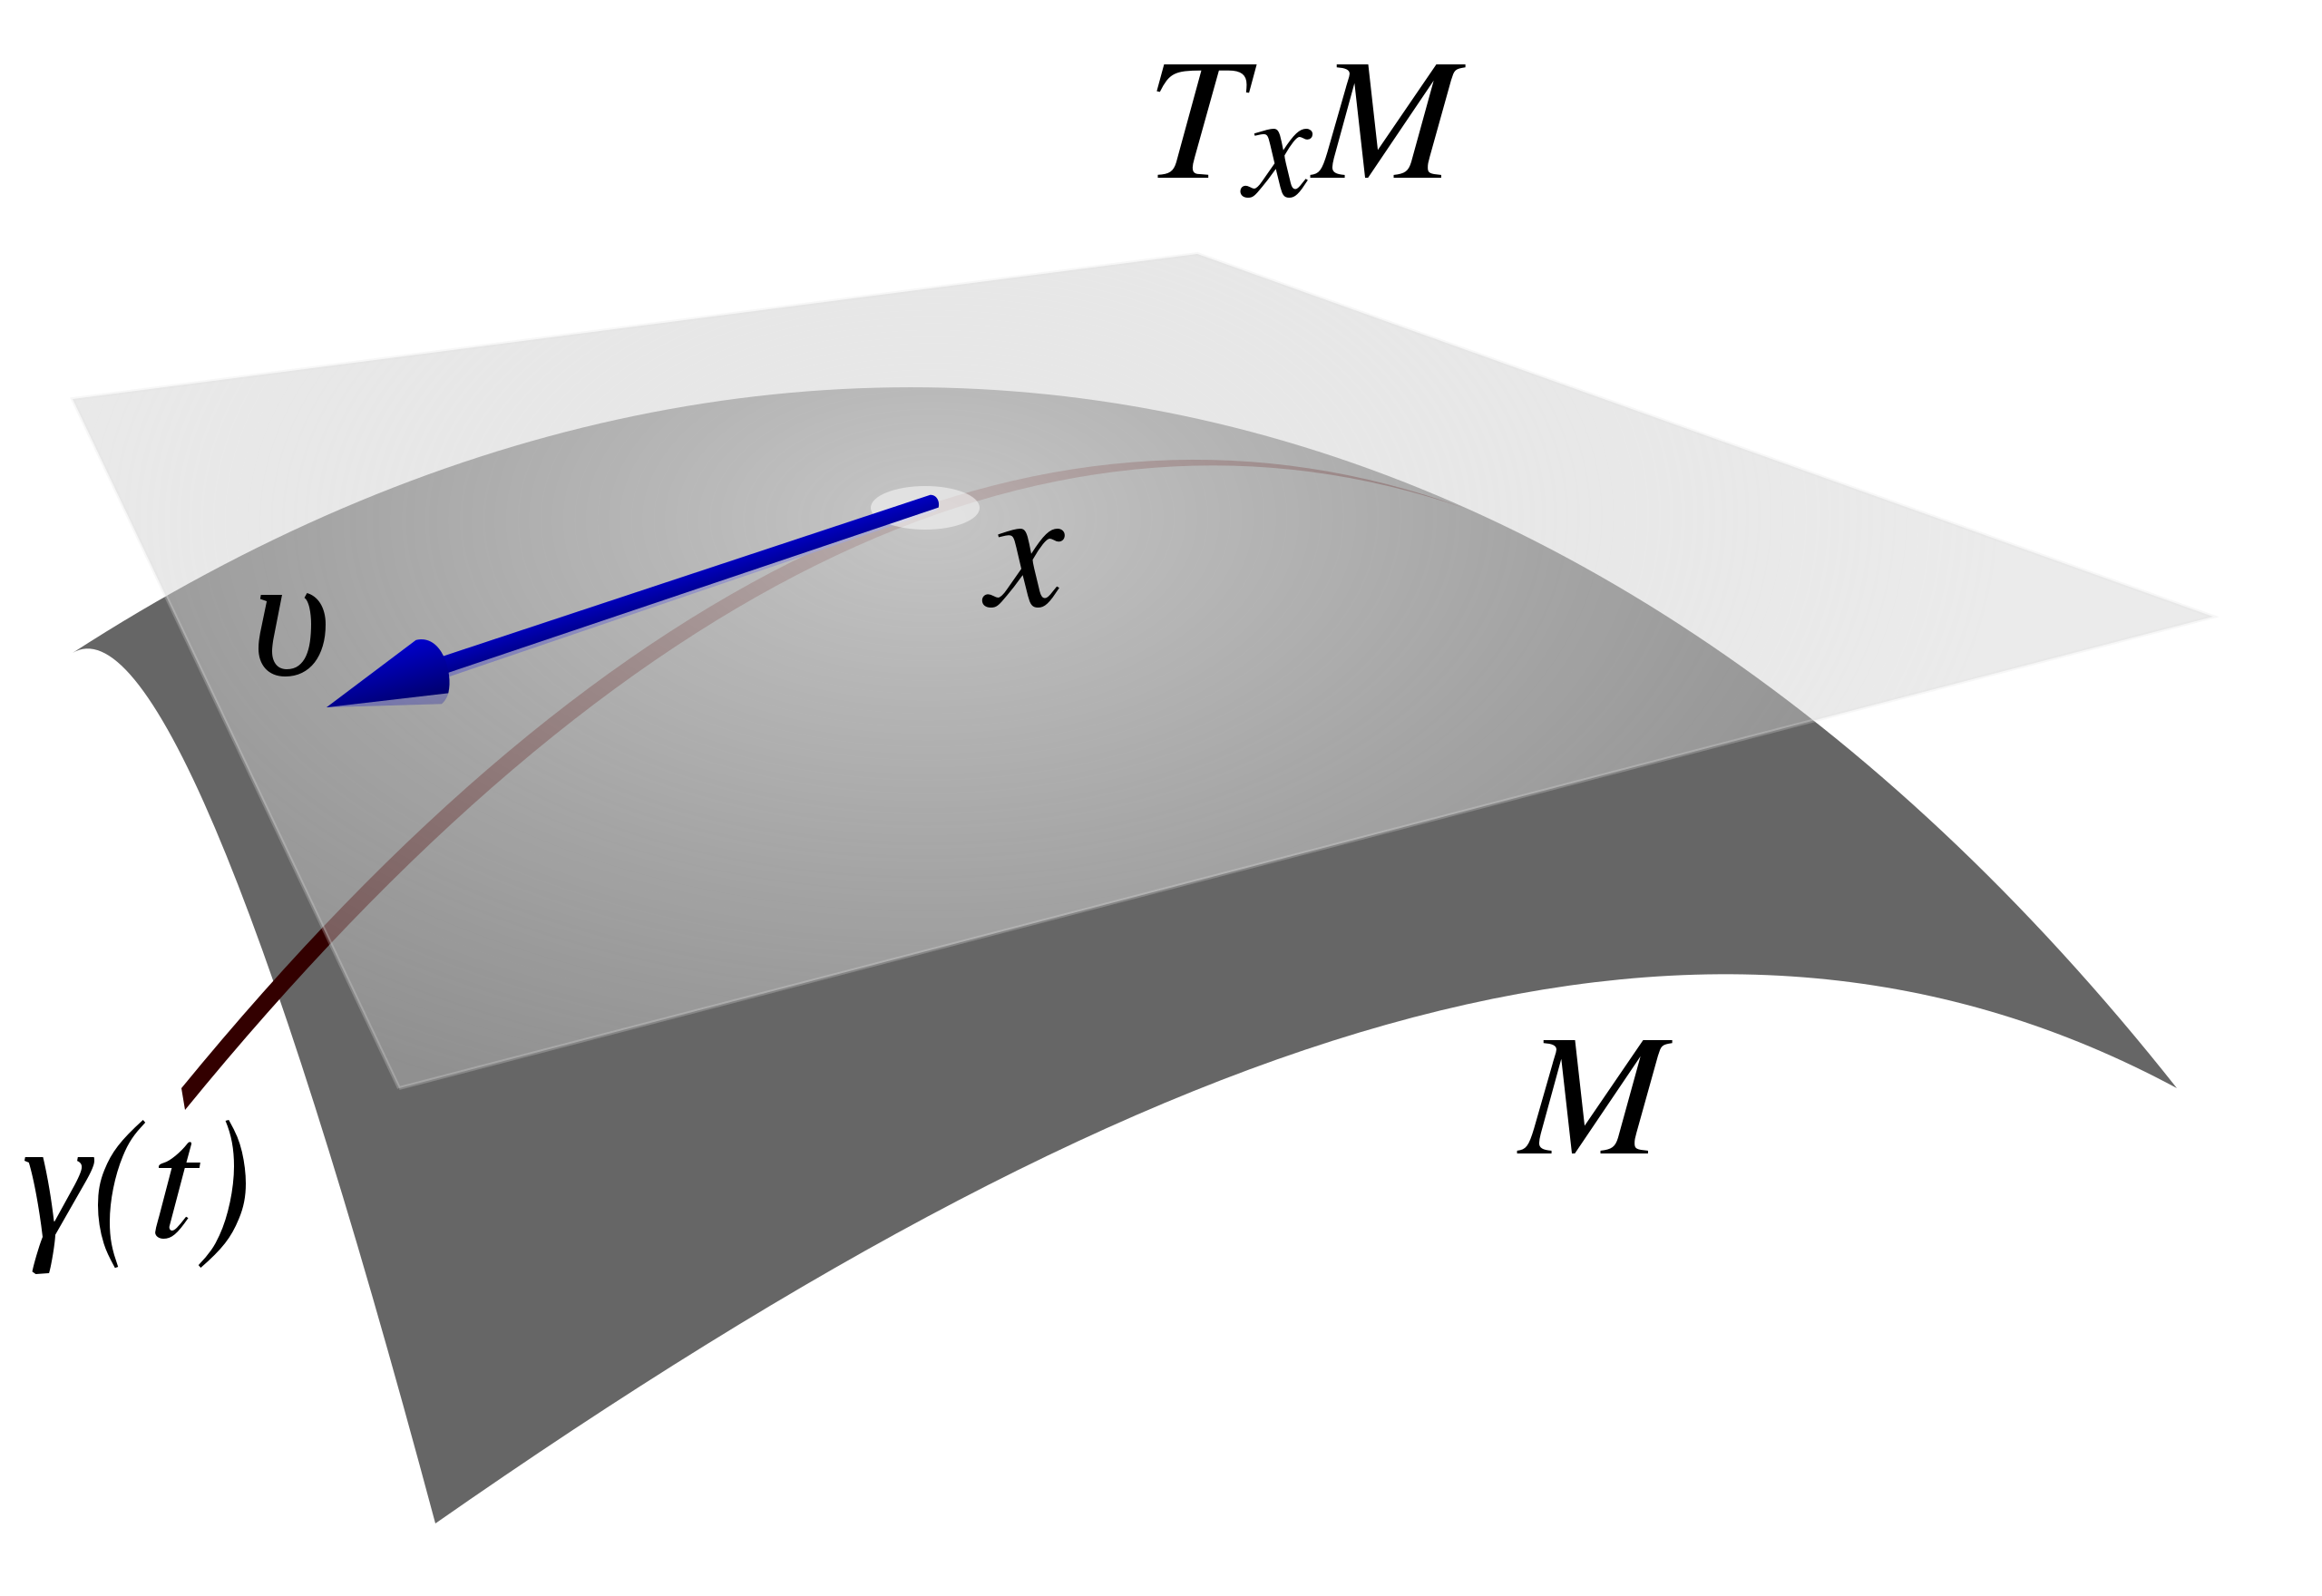
\includegraphics[width=.4\textwidth]{TACA_2019/tangent_space.png}
    \caption{A curve $\position$, its tangent vector $\velocity=\mathbf{v}$, and the tangent space $T_xM$.}
    \label{fig:tangent_space}
\end{figure}
\end{fig}

Then we wish to collect each of the tangent spaces along with the point at which they are attached.  Keeping track of the position we glue these vector spaces is very necessary as we will want to refer to elements in a specific tangent space.

\begin{df}{Tangent Bundle}{tangent_bundle}
The \textbf{tangent bundle}, $TM$, is the disjoint union of all the tangent spaces
\[
TM\coloneqq \bigsqcup_{x\in M} T_xM
\]
along with a projection map $\pi$ to the base space $M$.  We define $\pi$ so that for any $\mathbf{v}\in T_xM$ we have $\pi(\mathbf{v})=x$. 
\end{df}

Seeing an explicit example of a tangent bundle can help build intuition.  However, the tangent bundle can only be visualized easily on $1$-dimensional manifolds as $\dim(TM)\coloneqq 2\dim(T_xM)=2\dim(M)$. So even for $2$-dimensional manifolds, $\dim(TM)=4$. 

\begin{fig}{Building the Tangent Bundle}{build_tan_bundle}
\begin{figure}[H]
    \centering
    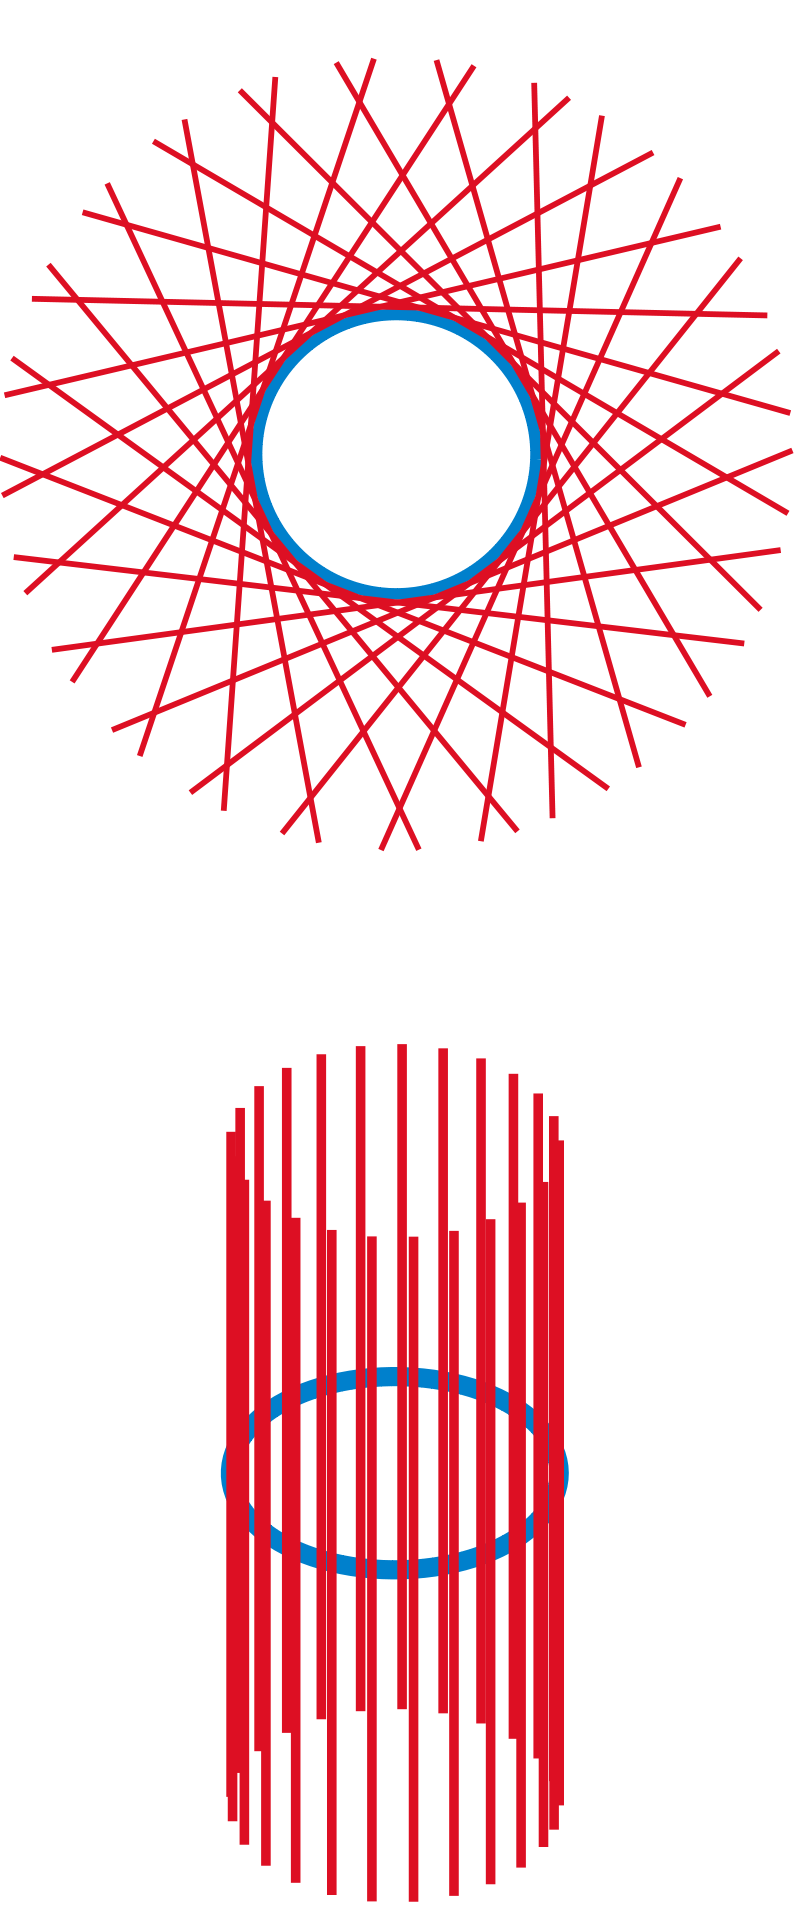
\includegraphics[width=.3\textwidth]{TACA_2019/s^1_tangent_bundle.png}
    \caption{(Top) Many different tangent spaces on the circle $S^1$. (Bottom) Reorienting the tangent spaces of $S^1$ to realize $TS^1=S^1\times \R$.}
    \label{fig:tangent_bundle}
\end{figure}
\end{fig}

We would like to also define the dual bundle to the tangent bundle so that we can later build tensors.  The idea used here will be helpful as well.

\begin{df}{Cotangent Bundle}{cotangent_bundle}
Let $TM$ be the tangent bundle.  Then we have that $T_xM=\pi^{-1}(x)$ which has has a dual vector space $T_x^*M$ we call the \textbf{cotangent space}.  Then the \textbf{cotangent bundle}, $T^*M$, is defined to be
\[
T^*M \coloneqq \bigsqcup_{x\in M} T_x^*M
\]
which sits over $M$ with projection $\pi$. 
\end{df}

\subsection{Sections of Bundles}
The point of defining sections is to properly generalize the notion of functions to manifolds. Specifically, sections are useful for defining vector (or tensor) valued functions on a manifold. The key issue is that, in general, manifolds may have not have global coordinates.  Thus we must be careful to build global functions in the correct way.

\begin{df}{Sections of Bundles}{sections_of_bundles}
Let $E$ be a vector bundle.  Then a (smooth) \textbf{section} $\sigma$ of $E$ is a (smooth) map
\[
\sigma \colon M \to E
\]
satisfying $\pi \circ \sigma = \id_M$. We then define the space of smooth sections
\[
\Gamma(E)\coloneqq \{\sigma ~\vert~ \textrm{$\sigma$ is a smooth section}\}.
\]
\end{df}

Visualizing a section of a bundle is not much more difficult.  In fact, a section is just a nice generalization of functions we have all seen in multivariate calculus.  Below is an example taking $M=S^1$ as our manifold. 

% Tangent Bundle and Section Picture

\begin{fig}{Sections of the Tangent Bundle}{sections_of_tan_bundle}
\begin{figure}[H]
    \centering
    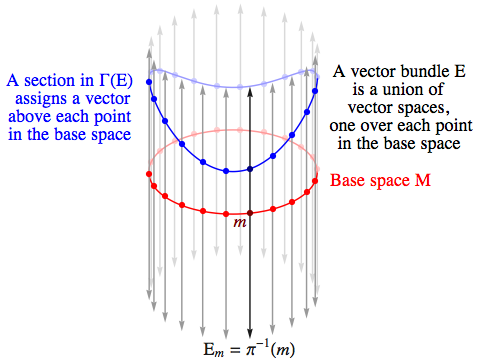
\includegraphics[width=.6\textwidth]{TACA_2019/s1_tan_bundle.png}
    \caption{Orienting the tangent spaces vertically, we can create the tangent bundle for $S^1$ as a product $TS^1=S^1\times \R$. A section of the tangent bundle is simply a smooth closed curve on $TS^1$ that moves around the circle component in a monotone way.}
    \label{fig:tangent_bundle_sec}
\end{figure}
\end{fig}

\begin{rmk}{Vector Fields are Sections}{vect_fields_sec}
The way we define a vector field on a manifold has essentially already been written down. A \textbf{vector field} is a section of the tangent bundle. We usually define the space of vector fields $\mathfrak{X}(M)$ by putting
\[
\mathfrak{X}(M)\coloneqq \Gamma(TM).
\]
\end{rmk}

% Stuff on Lie groups
% One may ask for more algebraic structure on manifolds or bundles.  This is the direction I wish to go in. Ultimately, I'd like to define a geometric (Clifford) algebra on a manifold.  The route requires this understanding of bundles.  A good start is to study manifolds that have an algebraic structure themselves. It turns out that \emph{Lie groups} serve this purpose well and are very rich in their own right.\\

% \begin{df}{Lie Group}{lie_gp}
% A \textbf{Lie group} $(G,\bullet)$ is a smooth manifold with a group structure.  We require the map $\bullet \colon G\times G \to G$ to be a smooth map.
% \end{df}

\subsection{Tensor Product of Bundles}

Geometers like to make measurements on spaces.  In the real world, all measurements we make come in the form of a real number.  Hence, this definition that follows should seem reasonably motivated. Another specific application of tensors on manifolds is to give a manifold shape.  If we just care about differentiable manifolds, we are working in the realm of differential topology.  In that respect, the unit sphere $S^2$ in $\R^3$ is no difference than the surface of a bumpy potato.

\begin{df}{(p,q)-Tensor}{pqtensor}
A \textbf{$(p,q)$-tensor} $\tau$ is a multilinear map
\[
\tau\colon \underbrace{V^*\times \cdots \times V^*}_{\textrm{$p$ copies}}\times \underbrace{V\times \cdots \times V}_{\textrm{$q$ copies}} \rightarrowtail \R.
\]
\end{df}

Then we collect all of the tensors on a vector space and place them in their own vector space.

\begin{df}{Tensor Space}{tensor_space}
We define the vector space $V^p_q$ of $(p,q)$-tensors on $V$ by writing
\[
\underbrace{V\otimes \cdots \otimes V}_{\textrm{$p$ copies}} \otimes \underbrace{V^*\otimes \cdots \otimes V^*}_{\textrm{$q$ copies}} \coloneqq \left\{ \tau ~\vert~ \textrm{$\tau$ is a $(p,q)-$tensor}\right\}.
\]
\end{df}

The question is then how to define tensor products of vector bundles.  Given a vector bundle $E$, we know that for each $x\in M$, $\pi^{-1}(x)=V$ is a vector space.  This leads us to a construction along each fiber. 

\begin{df}{Tensor Product of Bundles}{tensor_prod_bundle}
Let $(E,M,\pi_E)$ and $(F,M,\pi_F)$ be vector bundles over the same base manifold $M$.  Then we have for $x\in M$, $\pi_E^{-1}(x)=V$ and $\pi_F^{-1}(x)=W$ are the vector space fibers over the point $x$ in the respective bundles. The \textbf{tensor product of $E$ and $F$} is defined by
\[
E\otimes F \coloneqq \bigsqcup_{x\in M} \pi_E^{-1}(x)\otimes \pi_F^{-1}(x).
\]
\end{df}

\section{Parameterized Tensors}

With the framework built up, we can now realize tensors that are parameterized by a manifold.  Then are a few salient facts that should be mentioned.

\begin{df}{Tensor Field}{tensor_field}
A \textbf{$(p,q)$-tensor field} is a (smooth) section
\[
\tau \colon M \to \underbrace{T^*M\otimes \cdots T^*M}_{\textrm{$p$ copies}} \otimes \underbrace{TM\otimes \cdots \otimes TM}_{\textrm{$q$ copies}}.
\]
Equivalently, one can write
\[
\tau \in \Gamma(T^*M\otimes \cdots T^*M\otimes TM \otimes \cdots \otimes TM).
\]
In other words, at each point $x\in M$, $\tau(x)$ is a $(p,q)$-tensor.\\

\emph{Note:} We could have tensor fields that are constructed over different vector bundles, but the natural bundles on $M$ are $TM$ and $T^*M$.
\end{df}

The act of taking sections of a bundle $\Gamma(\cdot)$ plays nicely with the tensor product of bundles.  In fact, $\Gamma$ can be thought of as a functor in an appropriate sense.  This can be summed up in the following proposition and theorem. 

\begin{prop}{The Space of Sections is a Module}{sections_are_modules}
\emph{Let $E$ be a vector bundle. Then $\Gamma(E)$ is a $C^\infty(M)$-module.}
\end{prop}

It's worth noting that $\Gamma(E)$ is infinite dimensional. However, we will find that we still retain reflexivity.

Since we can realize the space of sections $\Gamma(E)$ as a module, this leads us to believe we can alternatively define tensor fields via taking tensor products of the modules of sections themselves.  This means of construction is potentially different.

\begin{thm}{Tensor Products of Sections}{tensor_product_section}
\emph{Let $E$ and $F$ be vector bundles over $M$.  Then we have}
\[
\Gamma(E)\otimes_{C^\infty(M)}\Gamma(F) = \Gamma(E\otimes F).
\]
\end{thm}

This shows that the two different constructions of a tensor field are equivalent and thus either are valid to work with.  At times, each has an advantage.  One last final result is in order.

\begin{thm}{Modules of Sections are Reflexive}{sections_reflexive}
\emph{Let $E$ be a vector bundle over $M$ and $\Gamma(E)$ be sections of the bundle. Then}
\[
\Gamma(E)^* = \Gamma(E^*).
\]
\emph{Hence, it follows that $\Gamma(E)$ is reflexive. That is,}
\[
\Gamma(E)^{**}=\Gamma(E^{**})=\Gamma(E)
\]
\emph{since $E$ is finite dimensional.}
\end{thm}

With all of this constructed, let us consider an extremely important example of all of this.  

\begin{ex}{Riemannian Manifold}{riemannian_manifold}
A \textbf{Riemannian manifold} $M\equiv(M,g)$ is a smooth manifold with a positive definite symmetric $(0,2)$-tensor field $g$. $M$ has many nice properties.
\begin{itemize}
    \item $M$ has an inner product on each $T_xM$.
    \item $TM$ and $T^*M$ are naturally isomorphic via Riesz representation.
    \item $M$ is a metric space.
    \item $M$ has a canonical volume form.
    \item $M$ has a natural connection on $TM$.
    \item $M$ has a well defined Laplacian on $k$-forms.
\end{itemize}
\end{ex}

Riemannian manifolds are extremely useful in generalizing calculus on $\R^m$ as they essentially mimic all of the structure in $\R^m$ aside from potentially having nontrivial topology or curvature.  On top of that, it is not asking much to build a Riemannian manifold since every smooth manifold admits a Riemannian metric.









\end{document}
